\chapter{Introduction, Background \& Objectives}

%This section should discuss your preparation for the project, including background reading, your analysis of the problem and the process or method you have followed to help structure your work.  It is likely that you will reuse part of your outline project specification, but at this point in the project you should have more to talk about. 

%\textbf{Note}: 

%\begin{itemize}
  % \item All of the sections and text in this example are for illustration purposes. The main Chapters are a good starting point, but the content and actual sections that you include are likely to be different.
   
   %\item Look at the document on the Structure of the Final Report for additional guidance. 
   
%\end {itemize}

%Outline:
%What problem was tackled?
%Why was that problem tackled?
%How (in outline) was the problem tackled?
%Clear statement of project aim and objectives
%Guide to subsequent chapters
%Usually drafted early, and finished last

\section{Introduction}
%\section{Background}
%What was your background preparation for the project? What similar systems did you assess? What was your motivation and interest in this project?
\textbf{NOTES: - DELETE THIS -}
\begin{itemize}
\item Route-planning applications are widely used.
\item PRMs not considered by most route-planners.
\item PRMs often find navigation hard (reference).
\item More PRMs in university (reference).
\item Aberystwyth University wants to make its campuses more accessible - ramps, automatic doors, etc.
\item Project builds upon BSc project (2015) and is inspired by Access Aber (summer 2014).
\end{itemize}


Route planning has been a useful tool for thousands of years; even before we started drawing maps, and routes were planned relative to landmarks and star-constellations. In our modern society, route-planning systems are becoming increasingly more accurate and commonplace in our daily lives. These systems can be used by anyone: From tourists trying to find the nearest public toilet, to the Mars rovers\cite{marsRover} - boldly going where no one has gone before.

A significant amount of money and effort has been put into extensively mapping our world \cite{OSM,gmaps1,gmaps2,geofabrik}, which in turn has provided route-planning systems even more data to work with -- making them more accurate and useful than ever before.

Route-planning systems are of course only practical to use if they are able to plan routes that their users are able to follow, which is unfortunately often not the case for persons with reduced mobility (PRM). Most public route-planning systems focus on providing routing-services to very large, generalised groups of people - like pedestrians, cyclists and cars, but very rarely consider PRMs as a separate group to these.

PRMs are often categorised as pedestrians, and are therefore given routes intended for people who are able to walk up stairs, cross streets with elevated curbs, climb steep hills, etc. Many PRMs are able to pass these obstacles with some assistance from someone else, but this does not apply to everyone; their wheelchair might be too heavy to lift manually, they might be old and/or have a form of muscular atrophy that makes it hard to walk, or there might not be anyone around to give them the help they need.

A PRM could try following routes intended for cyclists, as these usually avoid stairs, but they might still face tall curbs, paths with bad surfaces, steep slopes, etc. Bike-routes also tend to be noticeably longer than pedestrian routes, so these may not always be suitable for many PRMs either.

As built-up areas are often particularly challenging environments to navigate for PRMs, the project developed as part of this dissertation has focused most of its attention to areas like this. Additionally: Because Aberystwyth University has made a notable effort to make its campuses more accessible for everyone in recent years, and because there are more people with disabilities in higher education now than ever before\cite{tinklin2004}, this project has put its main focus on the Aberystwyth University campuses.

This project builds upon the author's Major project for their BSc degree at Aberystwyth University (\textquotedblleft Access Aber - Pathfinding\textquotedblright), completed in 2015, which in turn was inspired by a separate system developed by Aberystwyth University in the summer of 2014: \textquotedblleft Access Aber\textquotedblright.

\begin{figure}
	\centering
	
	
	\subfigure[Route for Persons with Reduced Mobility]{\frame{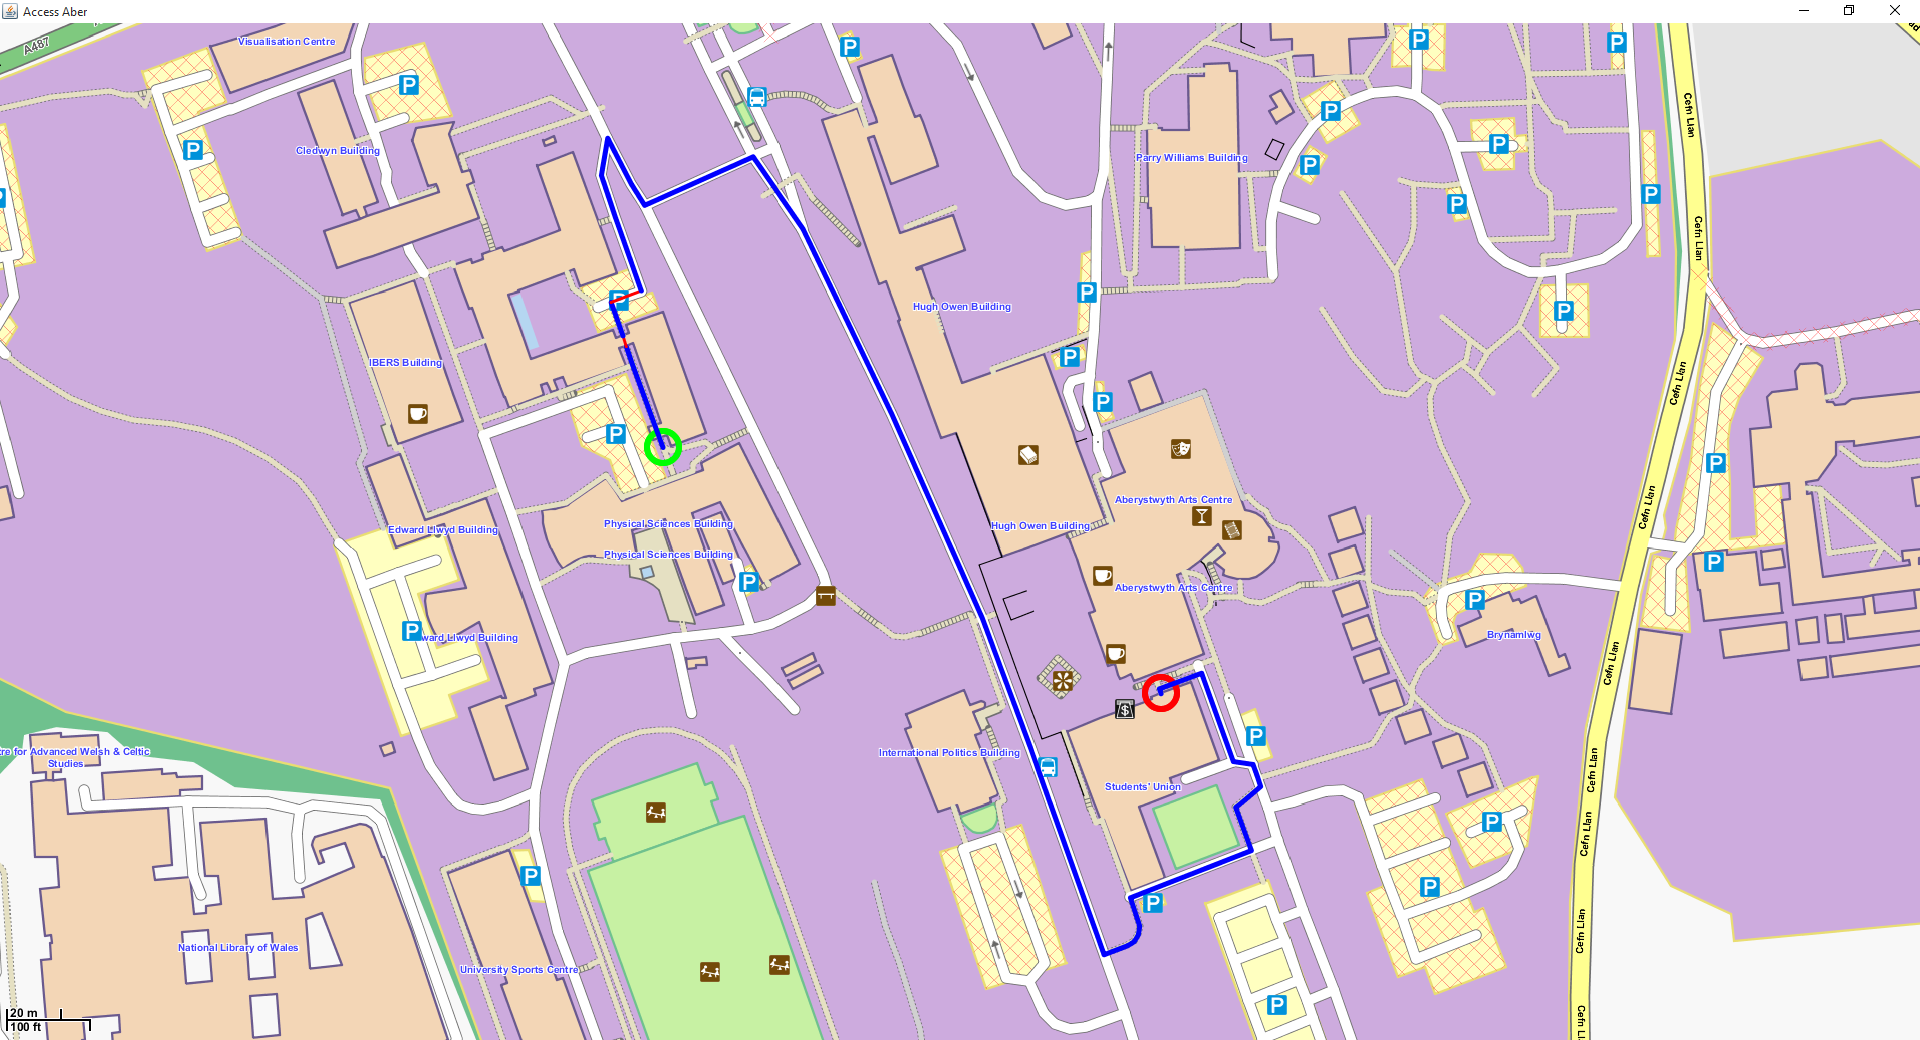
\includegraphics[keepaspectratio, width=\columnwidth]{Images/AStar_CSdept-SU}}}
	
	\subfigure[Route for able-bodied pedestrians]{\frame{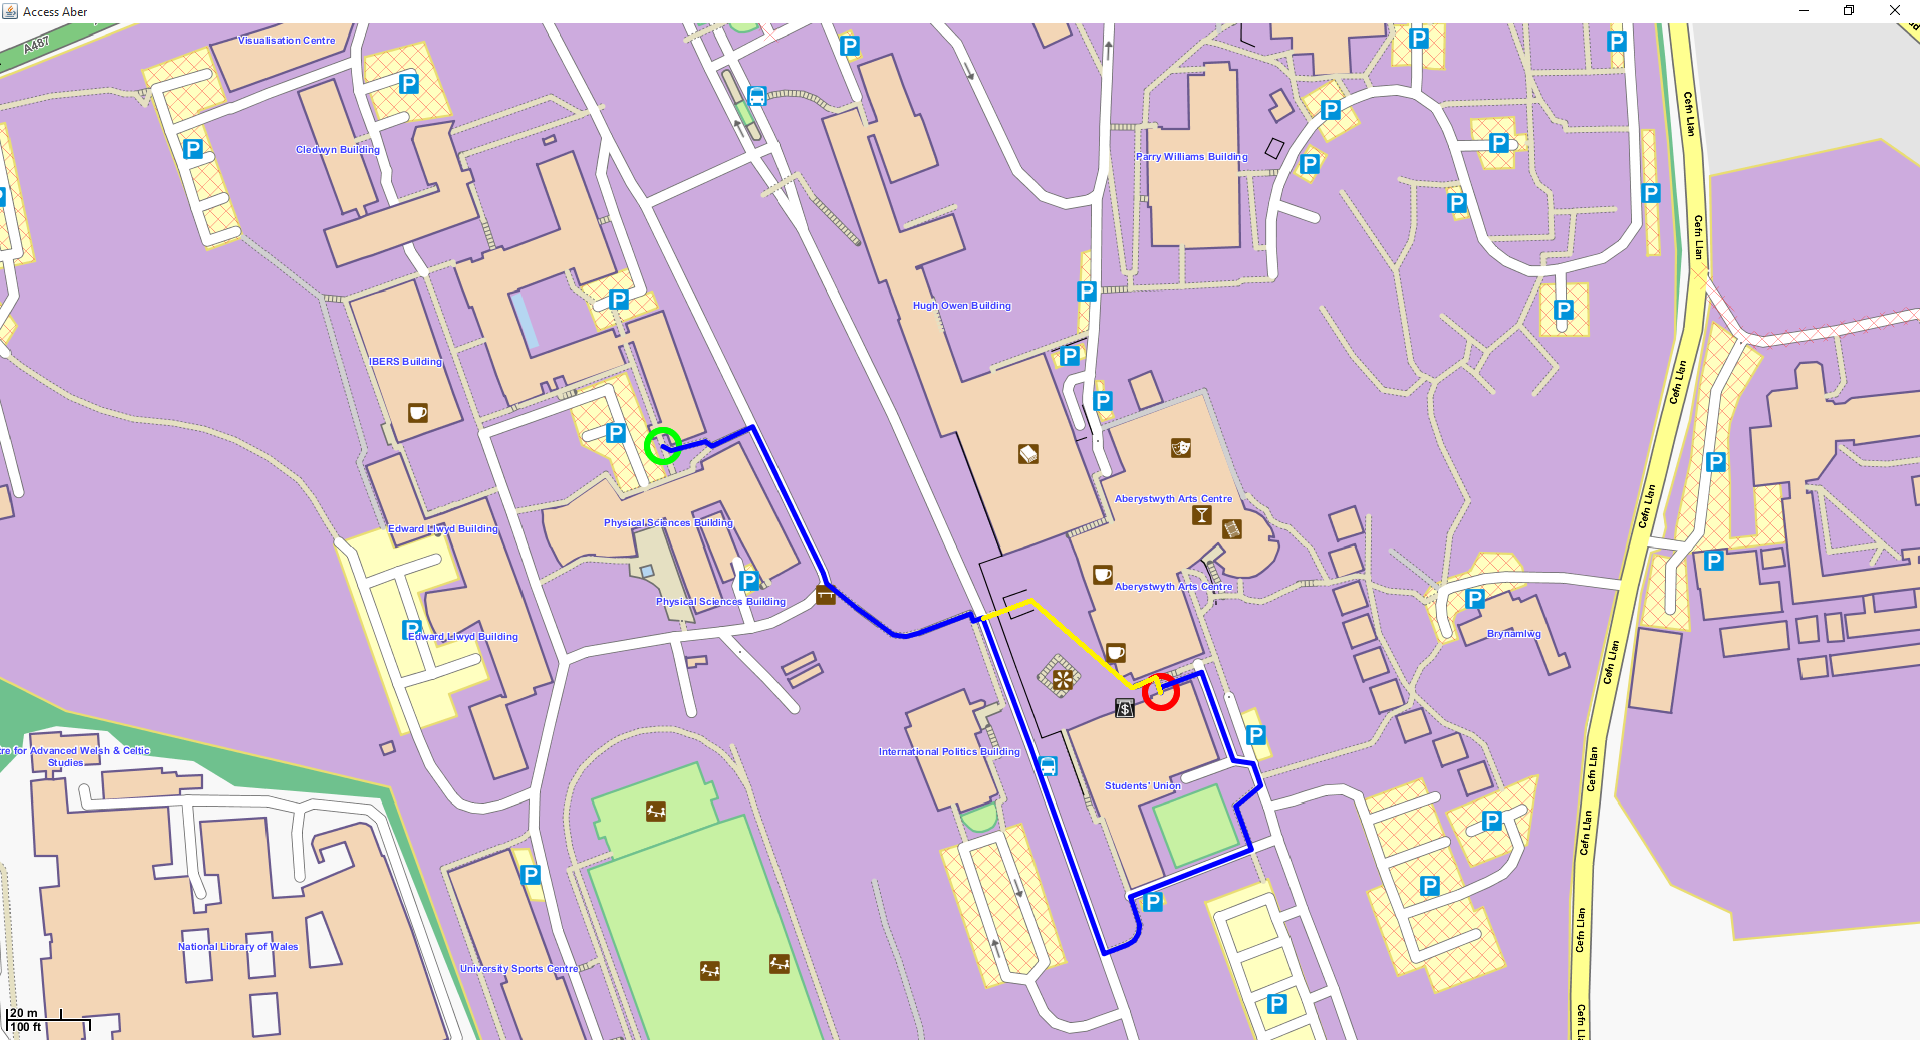
\includegraphics[keepaspectratio, width=\columnwidth]{Images/AStar_CSdept-SU_Foot}}}
	\caption[Longer routes for Persons with Reduced Mobility]{These images show the route some PRMs would need to follow to get from the computer-science department (\textit{IMPACS}) on Penglais campus, to the Students' Union. As there are many stairs in the way, many PRMs are forced to follow a far longer route than an able-bodied person would. The yellow line in (b) (hand-drawn by me -- starting where (a) and (b) intersect) shows the actual path an able-bodied pedestrian would take. The route in (b) is sub-optimal because data is missing from the OSM-database; Mapzen on \url{openstreetmap.org} finds the same route as (b) (29.September.2016), so the fault is most likely in the OSM-database.}
	\label{fig:longerRoutePRM}
\end{figure}

\section{Project aims}
%\section{Analysis}
%Taking into account the problem and what you learned from the background work, what was your analysis of the problem? How did your analysis help to decompose the problem into the main tasks that you would undertake? Were there alternative approaches? Why did you choose one approach compared to the alternatives? 

%There should be a clear statement of the objectives of the work, which you will evaluate at the end of the work. 

%In most cases, the agreed objectives or requirements will be the result of a compromise between what would ideally have been produced and what was felt to be possible in the time available. A discussion of the process of arriving at the final list is usually appropriate.
\textbf{NOTES: - DELETE THIS -}
\begin{itemize}
	\item Make it clear that PRMs need to be considered by more route-planners.
\\
	\item Find optimal and complete algorithm(s).
	\item Algorithm(s) have to plan routes in near-real-time.
	\item Algorithm(s) have to use as little memory as possible.
	\item Algorithm(s) needs to be able to distinguish between accessible and inaccessible paths.
	\item Make a process for automatically filtering out Nodes and Ways deemed unsuitable for navigation.
\\
	\item Investigate how to store, represent and index the OpenStreetMap database containing all of the Nodes and Ways to be used for pathfinding.
	\item Display the routes on a map. (is this really a project aim?).
\end{itemize}

The goal of this project is to show that it is possible to plan routes for PRMs, but more importantly: It is important to show that route-planners need to consider PRMs to a much larger degree than they currently do, and that some areas on Aberystwyth University's campuses could still be made more accessible than they currently are.

The system developed as part of this dissertation has to identify the most important aspects of route planning, and replicate this in a route-planning system made specifically for PRMs.
These aspects include, but are not limited to: calculating routes in near-real-time, having a low memory-footprint, employing optimal and complete routing-algorithms, and of course finding appropriate routes for the target users.

The process of extensive and accurate mapping of Nodes (or individual points of navigational data) is a task beyond the scope of this project, so this data will have to be retrieved from a third party. This will be discussed in more detail later in this report.

%TODO I removed this section - not sure what to write here
%\section{Objectives}
%\section{Process}
%You need to describe briefly the life cycle model or research method that you used. You do not need to write about all of the different process models that you are aware of. Focus on the process model that you have used. It is possible that you needed to adapt an existing process model to suit your project; clearly identify what you used and how you adapted it for your needs.

\section{Results}